\documentclass[10pt]{beamer}

%Paquets d'écriture et de compatibilité française
\usepackage[T1]{fontenc} 
\usepackage{lmodern}

%Paquets d'ajouts esthétiques
% Pour pouvoir aligner les images correctement
\usepackage{graphbox}
% Pour avoir les tableaux
\usepackage{tabularx}
% Pour faire des cellules de tableau
\usepackage{makecell}
% Gestion des images
\usepackage{graphicx}
% Gestion du thème
\usetheme{metropolis}
%\setbeameroption{show only notes}
%\setbeamercolor{progress bar}{
%	use=alerted text,
%	fg=blue,
%	bg=alerted text.fg!50!black!30
%}

\setbeamertemplate{frame footer}{\footnotesize\insertsection}
\setbeamerfont{alerted text}{series=\bfseries,size=\huge}

\metroset{numbering=fraction,block=fill,progressbar=frametitle}

\makeatletter
\setlength{\metropolis@titleseparator@linewidth}{1.5pt}
\setlength{\metropolis@progressonsectionpage@linewidth}{1.5pt}
\setlength{\metropolis@progressinheadfoot@linewidth}{1.5pt}

\setbeamertemplate{title page}{
	\begin{minipage}[b][\paperheight]{\textwidth}
		\ifx\inserttitlegraphic\@empty\else\usebeamertemplate*{title graphic}\fi
		\vfill%
		\ifx\inserttitle\@empty\else\usebeamertemplate*{title}\fi
		\ifx\insertsubtitle\@empty\else\usebeamertemplate*{subtitle}\fi
		\usebeamertemplate*{title separator}
		\vspace*{5mm}

		\begin{tabularx}{\textwidth}{Xr}
			\makecell[l]{
				\ifx\beamer@shortauthor\@empty\else\usebeamertemplate*{author}\fi\\
				\ifx\insertinstitute\@empty\else\usebeamertemplate*{institute}\fi
			}
		\end{tabularx}

		\vfill
		\vspace*{1mm}
	\end{minipage}
}

\setbeamertemplate{title}{
	\linespread{1.0}%
	\inserttitle%
	\par%
	\vspace*{0.5em}
}

\setbeamertemplate{subtitle}{
	\insertsubtitle%
	\par%
	\vspace*{0.5em}
}

\setbeamertemplate{author}{
	%\linespread{1.0}%
	\large{\insertauthor}%
	\par%
	\vspace*{0.5em}
}
\makeatother


\title{Workshop VIM}
\subtitle{Découverte et prise en main}
\author{MasterFox}

\begin{document}
\maketitle

\section{Vi : Les origines}
\begin{frame}{\textbf{C'est l'histoire de la Vi}}

	\center
	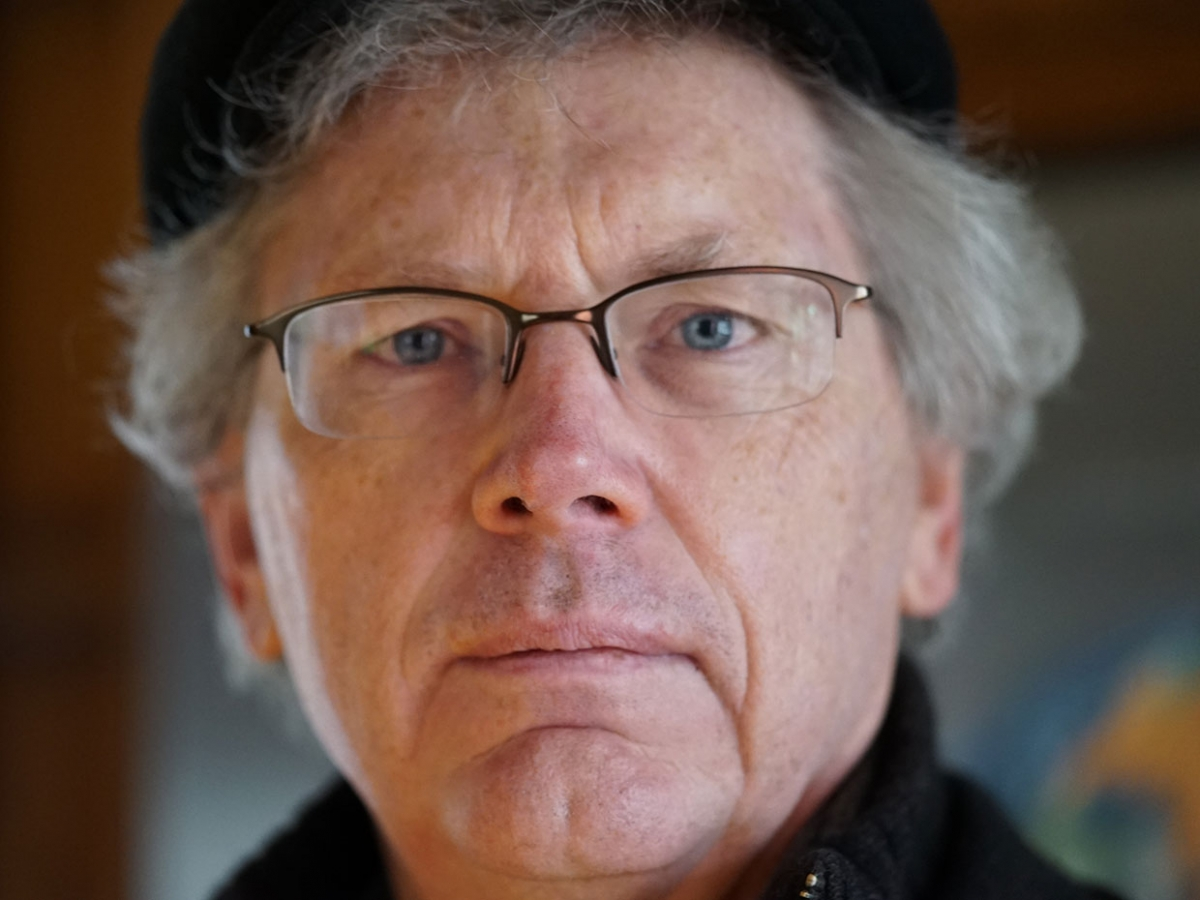
\includegraphics[height=96]{img/bill-joy.jpeg}
	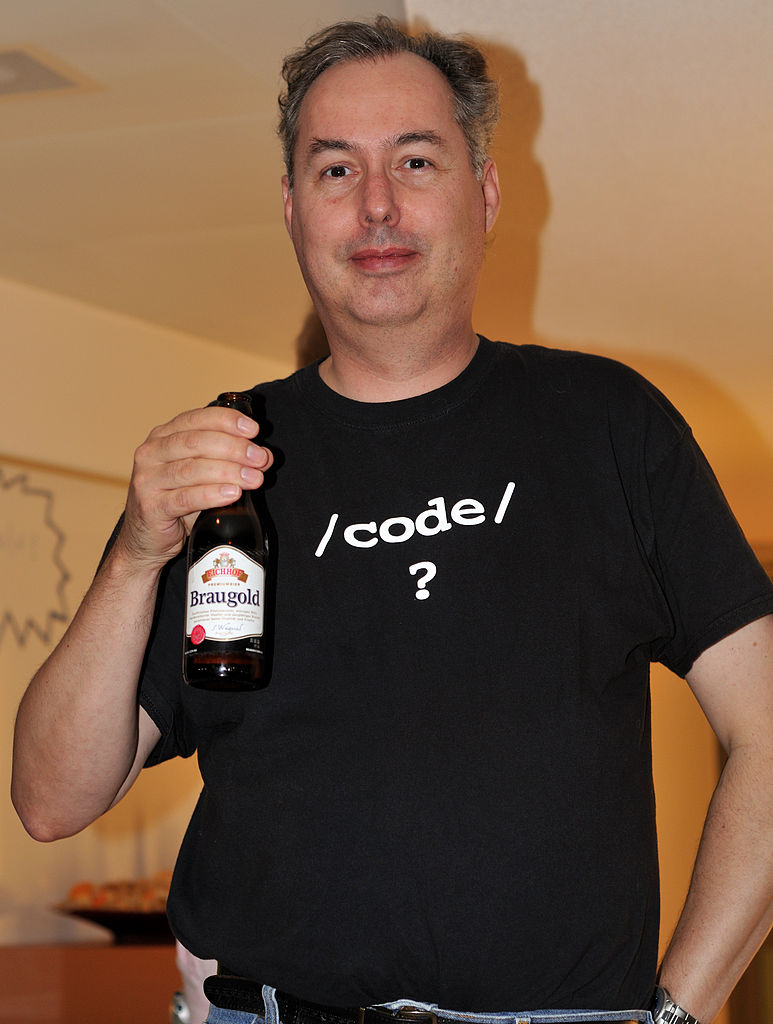
\includegraphics[height=96]{img/bram-moolenaar.jpg}

	%Tout commença en 1976
	Vi \rightarrow Vim \rightarrow Neovim\\
	\vspace{20pt}

	\raisebox{-0.5\height}{
\includegraphics[height=42]{img/logo-vim.png}}
	\hspace{10pt}
	\raisebox{-0.5\height}{
\includegraphics[height=42]{img/logo-neovim.png}}

\end{frame}

\section{Les bases}
	\begin{frame}{Comment ça marche}
		\center
		\huge 3 modes\\
		\vspace{5pt}
		\large Normal, Insertion, Visuel\\
		\vspace{10pt}
		\textbf{Il faut être normal !}\\
		\vspace{20pt}
		
\includegraphics[height=50pt]{img/example.png}
	\end{frame}

	\begin{frame}{Déplacements relatifs}
		\center
		\raisebox{-0.5\height}{
\includegraphics{img/control-keys.png}}
		\begin{tabular}{|c|c|}
			\hline
			\textbf{Mnemonique} & \textbf{Signification} \\ 
			\hline
			\hline
			w & word \\ 
			\hline
			e & end of word \\ 
			\hline
			b & backward \\ 
			\hline
			) & phrase \\ 
			\hline
			\} & paragraphe/fonction \\ 
			\hline
		\end{tabular}
		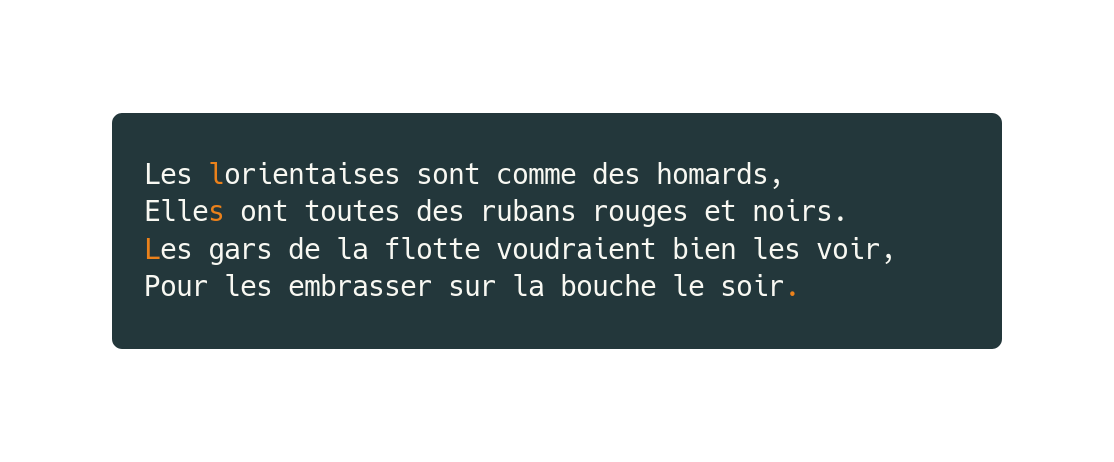
\includegraphics[width=256]{img/moves.png}
	\end{frame}

	\begin{frame}{Déplacements absolus}
		\begin{columns}[C]
			\begin{column}{0.50\textwidth}
				\center
				\begin{tabular}{|c|c|}
					\hline
					\textbf{Mnemonique} & \textbf{Signification} \\ 
					\hline
					\hline
					gg & Début de fichier \\ 
					\hline
					G & Fin de fichier \\ 
					\hline
					H & Haut de l'écran \\ 
					\hline
					M & Milieu de l'écran \\ 
					\hline
					L & Bas de l'écran \\ 
					\hline
				\end{tabular}

				\vspace{10pt}
				\Large Et \%
			\end{column}
			\begin{column}{0.47\textwidth}
				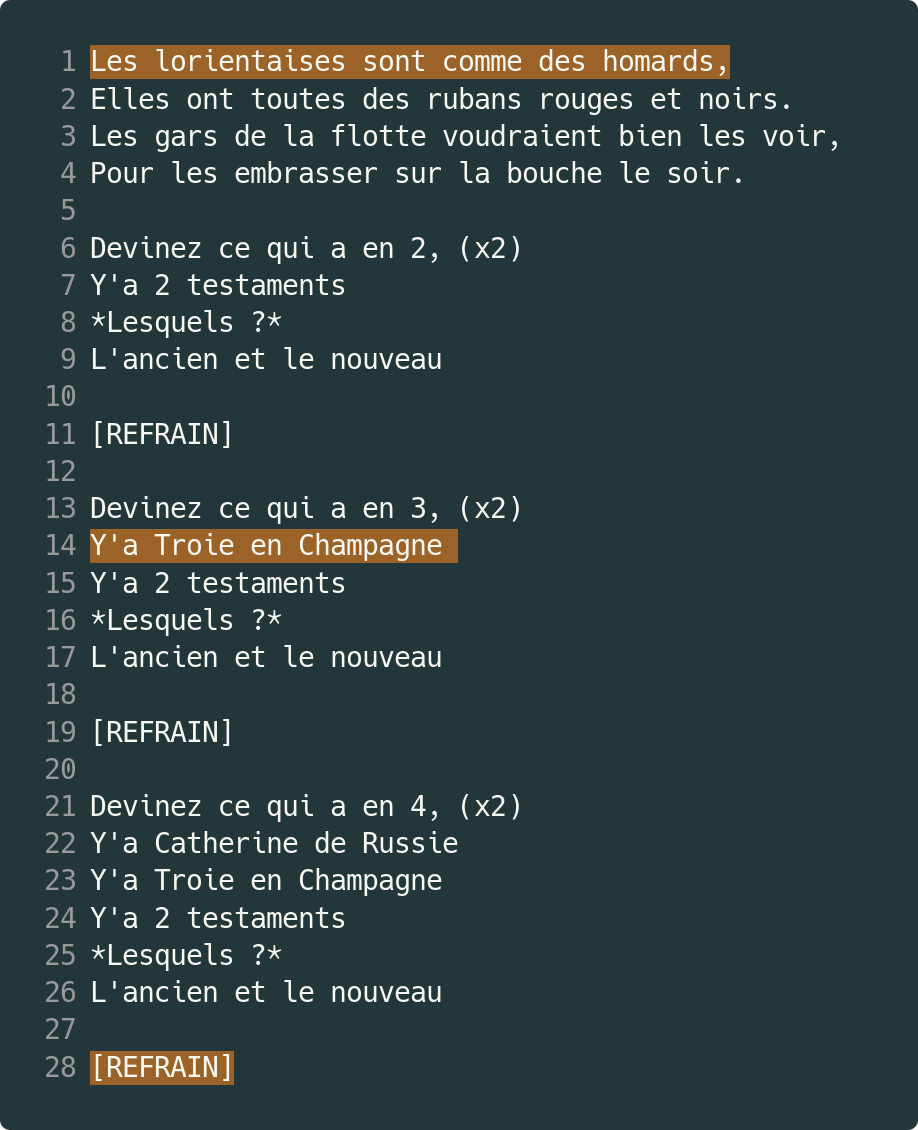
\includegraphics[width=160pt]{img/position.png}
			\end{column}
		\end{columns}

	\end{frame}

	\begin{frame}[standout]
		Jouons à un PETIT JEU !\\
		\vspace{10pt}
		
\includegraphics[width=48]{img/edit-vimrc.png}\\
		\vspace{10pt}
		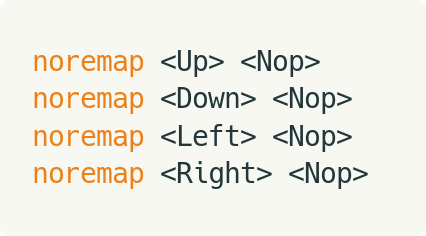
\includegraphics[width=128]{img/harder.png}
	\end{frame}

\section{Les registres}
	\begin{frame}{Keskessé}
		\begin{columns}[C]
			\begin{column}{0.50\textwidth}
				Des endroits de stockage, utilisés par:\\
				\begin{itemize}
					\item Le système
					\item Vim
					\item Vous
				\end{itemize}
			\end{column}
			\begin{column}{0.47\textwidth}
				
\includegraphics[width=96]{img/chest.jpg}
			\end{column}
		\end{columns}

		\vspace{5pt}
		Qui permettent de stocker "temporairement" des données.
	\end{frame}

	\begin{frame}{Les marques}
		\center
		
\includegraphics[height=100]{img/mark.jpeg}\\
		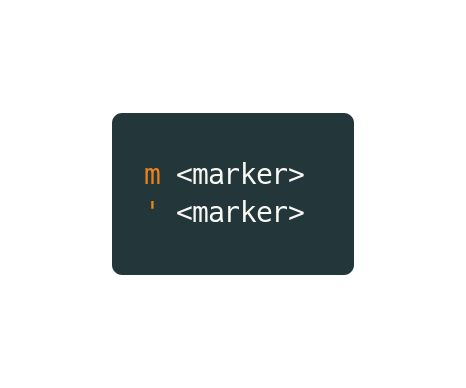
\includegraphics[height=100]{img/markers.png}
	\end{frame}

	\begin{frame}{Les macros}
		\center
		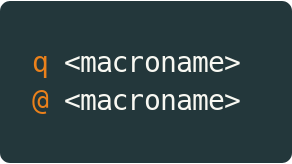
\includegraphics[height=50]{img/macros.png}
	\end{frame}

	\begin{frame}[standout]
		Des questions ?
	\end{frame}

\section{Vim power !}
	\begin{frame}{Les bases}
		\begin{columns}[C]
			\begin{column}{0.50\textwidth}
				\center
				% Salut les utilisateurs de tmux
				Afficher la page de manuel : K
				Refaire la dernière action : .
				Auto complétion : <C-n>
			\end{column}
			\begin{column}{0.47\textwidth}
				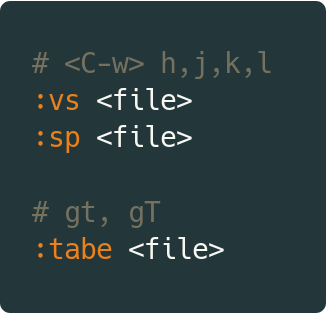
\includegraphics[height=100]{img/splittin.png}\\
			\end{column}
		\end{columns}
	\end{frame}

	\begin{frame}{Let's go flag}
		Utilisation de programmes externes\\
		ga, g8\\
		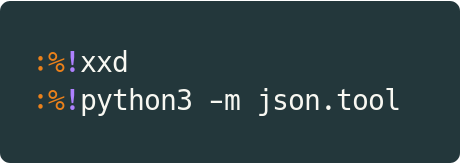
\includegraphics[height=32]{img/tools.png}\\
		%apérictf humans
	\end{frame}

	\begin{frame}{Let's \textit{r i c e}}
		%	Vim
		%	curl -fLo ~/.vim/autoload/plug.vim --create-dirs https://raw.githubusercontent.com/junegunn/vim-plug/master/plug.vim	
		%	Neovim
		%	curl -fLo ~/.local/share/nvim/site/autoload/plug.vim --create-dirs https://raw.githubusercontent.com/junegunn/vim-plug/master/plug.vim	
	\end{frame}

\begin{appendix}

	\begin{frame}[standout]
		Merci d'avoir écouté !
	\end{frame}

	\begin{frame}
		\frametitle{Sources}
		\begin{itemize}
				%Documentation
			\item \href{https://neovim.io/}{Neovim https://neovim.io/}
			\item \href{https://www.vim.org}{Vim https://www.vim.org}
			\item \href{https://vim.fandom.com/wiki/}{Wiki Vim https://vim.fandom.com/wiki/}
			\item \href{https://vimcolors.com/}{Vim Colorscheme https://vimcolors.com/}
			\item \href{https://vimawesome.com/}{Vim Awesome https://vimawesome.com/}
		\end{itemize}
	\end{frame}

	\begin{frame}[standout]
		Des questions ?
	\end{frame}

\end{appendix}
\end{document}
